



%%CHAP. Theory

\begin{figure}[h]
\centering
  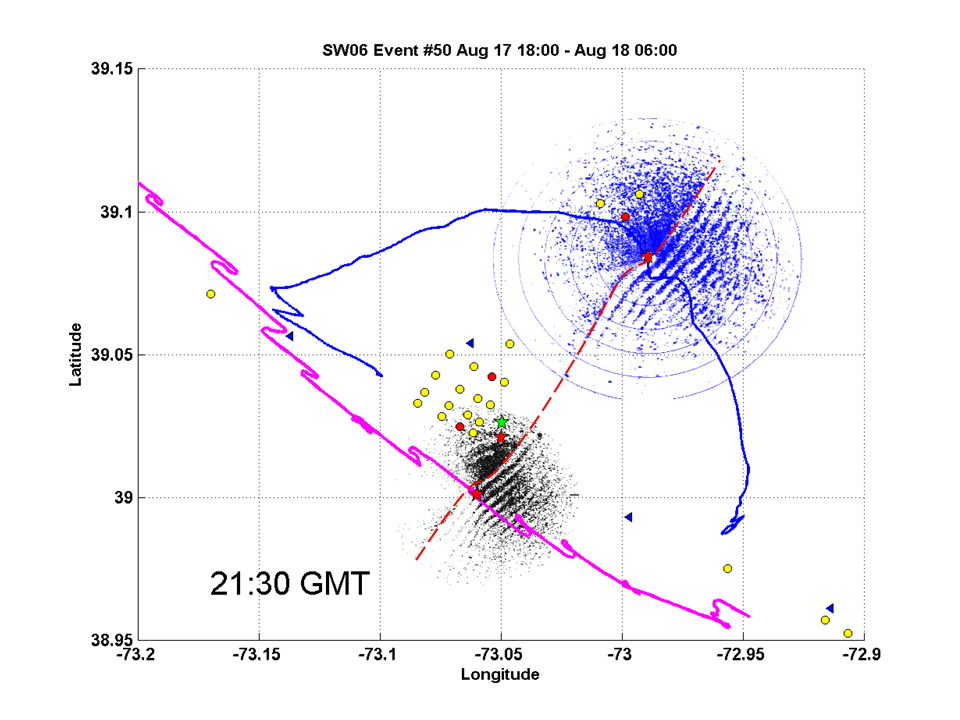
\includegraphics[width=0.8\textwidth]{IW_radar2.png}\\
  \caption{Radar image of internal wave surface signature at 21:30GMT . }
  \label{fig:IW_radar2}
\end{figure}

\begin{figure}[h]
\centering
  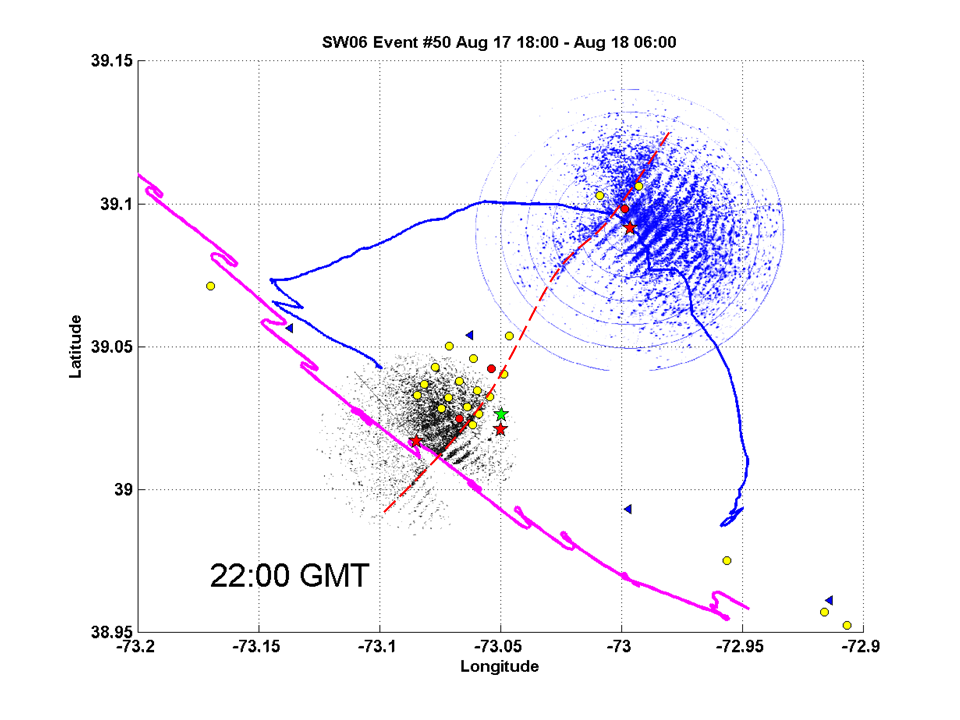
\includegraphics[width=0.8\textwidth]{IW_radar1.png}\\
  \caption{Radar image of internal wave surface signature at 22:00GMT . }
  \label{fig:IW_radar1}
\end{figure}

% \begin{figure}[h]
%\centering
 % 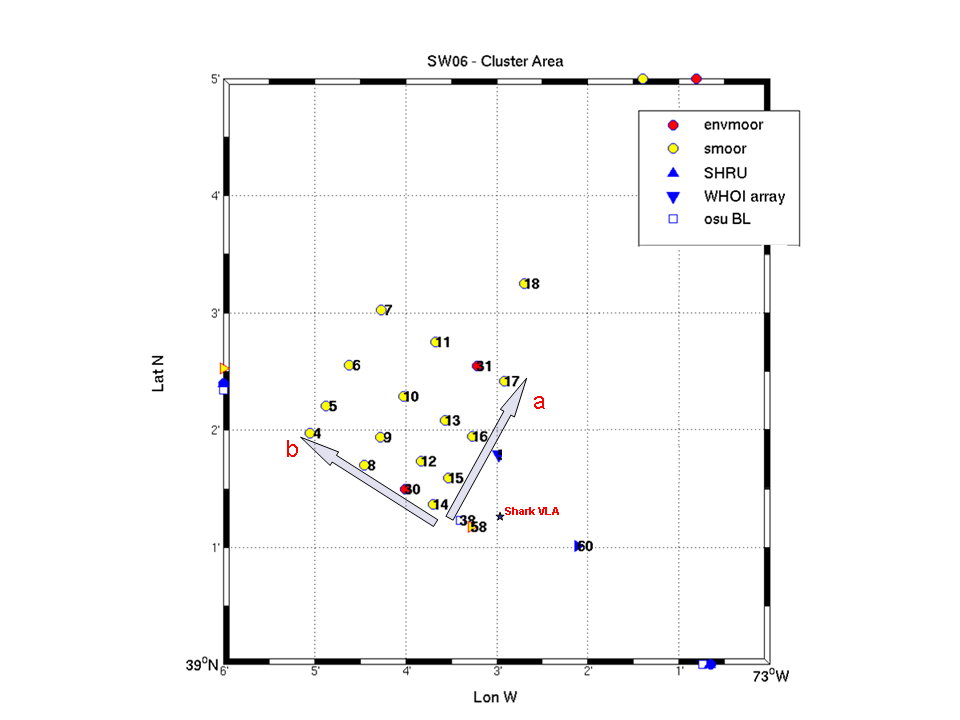
\includegraphics[width=0.8\textwidth]{T_farm2.png}\\
 % \caption{Thermistor farm deployed in SW06. Edge (a) \& (b) are parallel and perpendicular to the internal wave fronts, respectively. }
  %\label{fig:tfarm}
%\end{figure}

 \begin{figure}[h]
\centering
  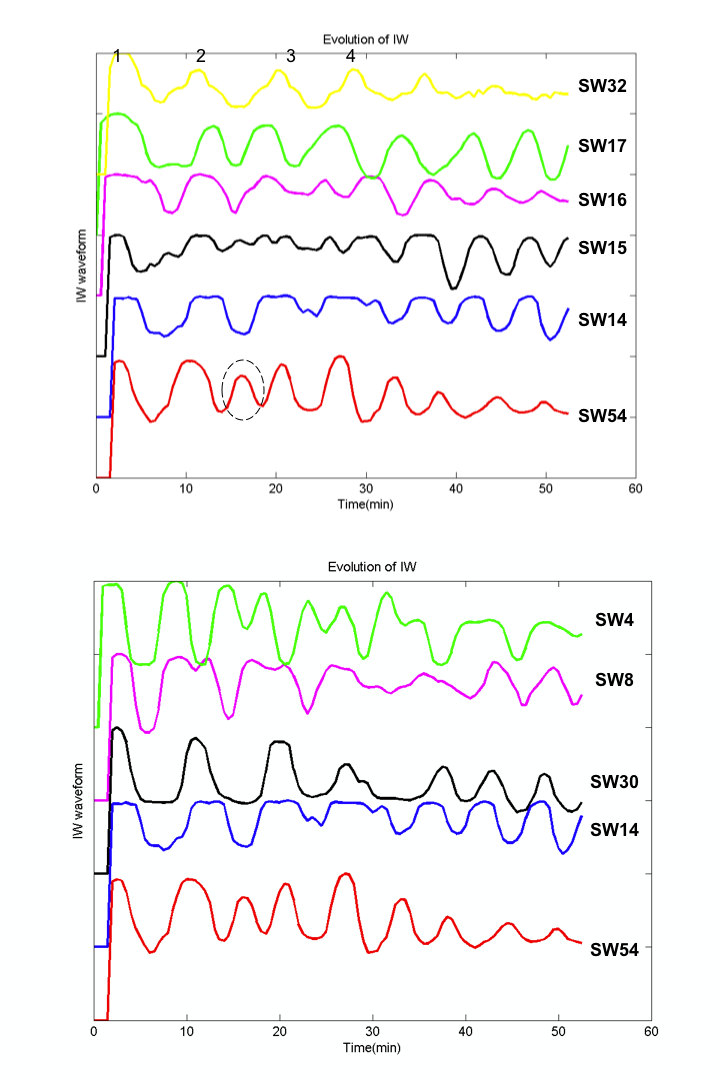
\includegraphics[width=0.8\textwidth]{tfarm_iw.png}\\
  \caption{Temperature data recorded by the thermistor farm during SW06 event 50. }
  \label{fig:tfarm_dir}
\end{figure}

\begin{figure}[h]
\centering
  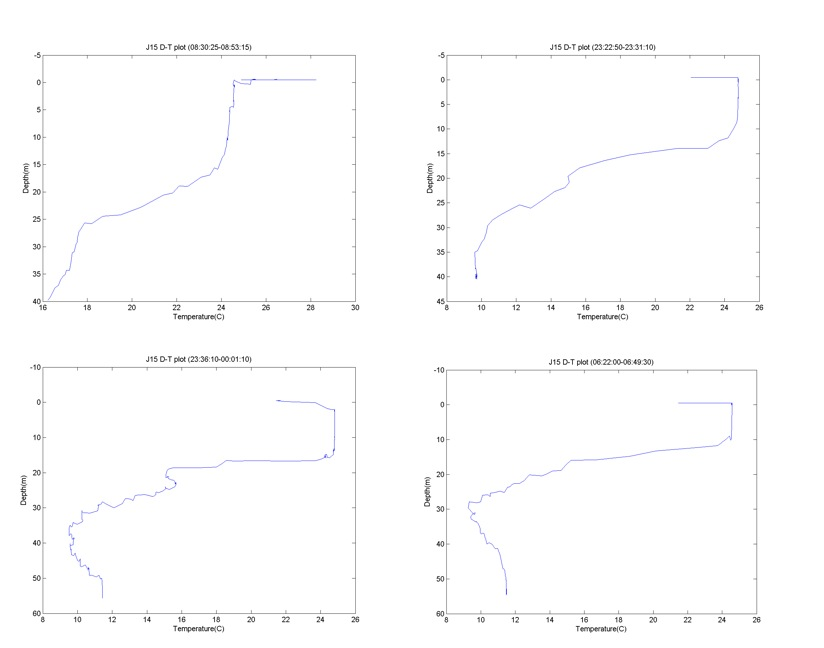
\includegraphics[width=0.8\textwidth]{water_temp4.jpg}\\
  \caption{Temperature profile recorded by TD sensor attached to J15 transducer}
  \label{fig:water_temp4}
\end{figure}

%\begin{figure}[h]
%\centering
  %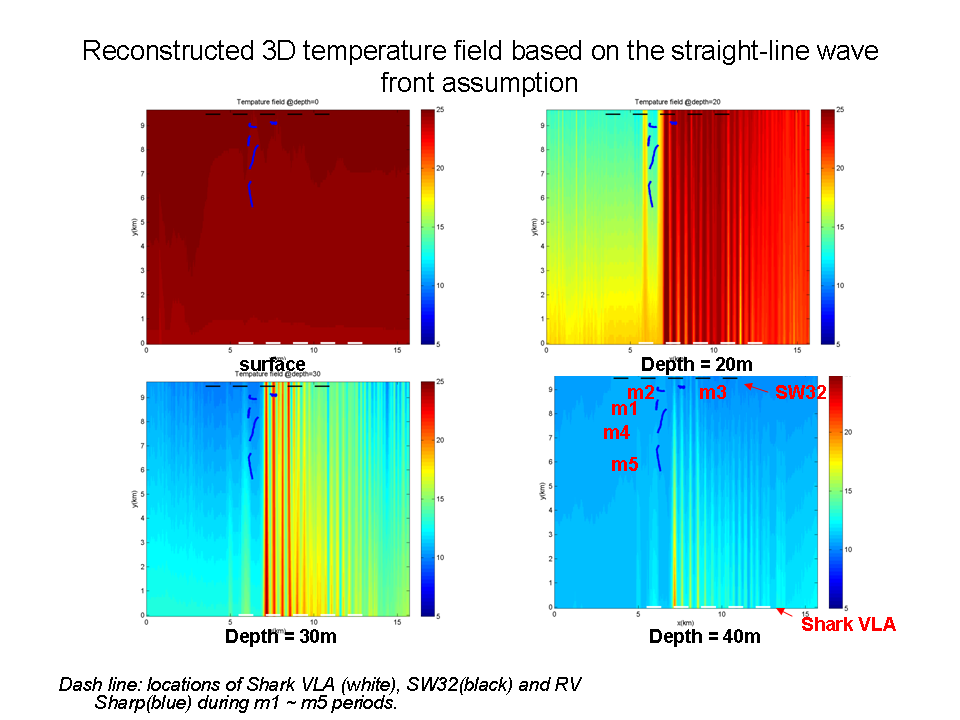
\includegraphics[width=0.8\textwidth]{3D_temp_recon.png}\\
  %\caption{Reconstructed temperature field and the movement of source and receiver in the internal wave coordinates}
  %\label{fig:water_temp4}
%\end{figure}

\begin{figure}[h]
\centering
  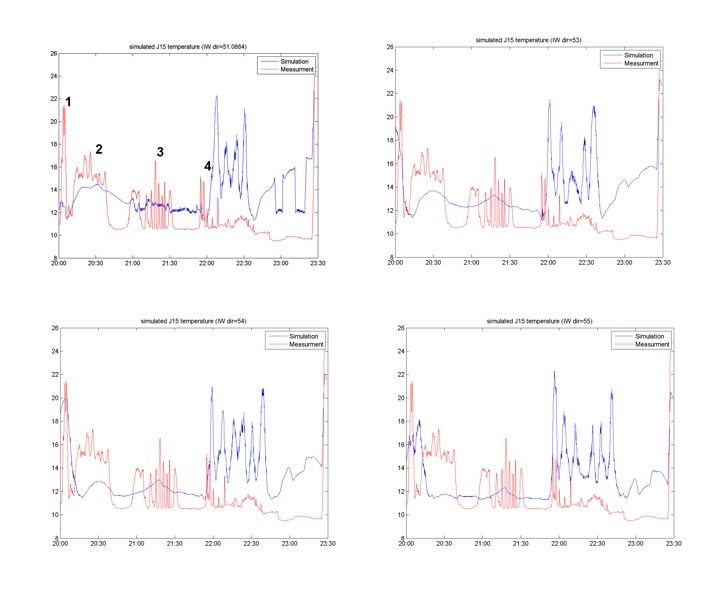
\includegraphics[width=0.8\textwidth]{J15_sim.jpg}\\
  \caption{Simulated J15 recored in reconstructed 3D environment}
  \label{fig:water_temp4}
\end{figure}

%\begin{figure}[h]
%\centering
  %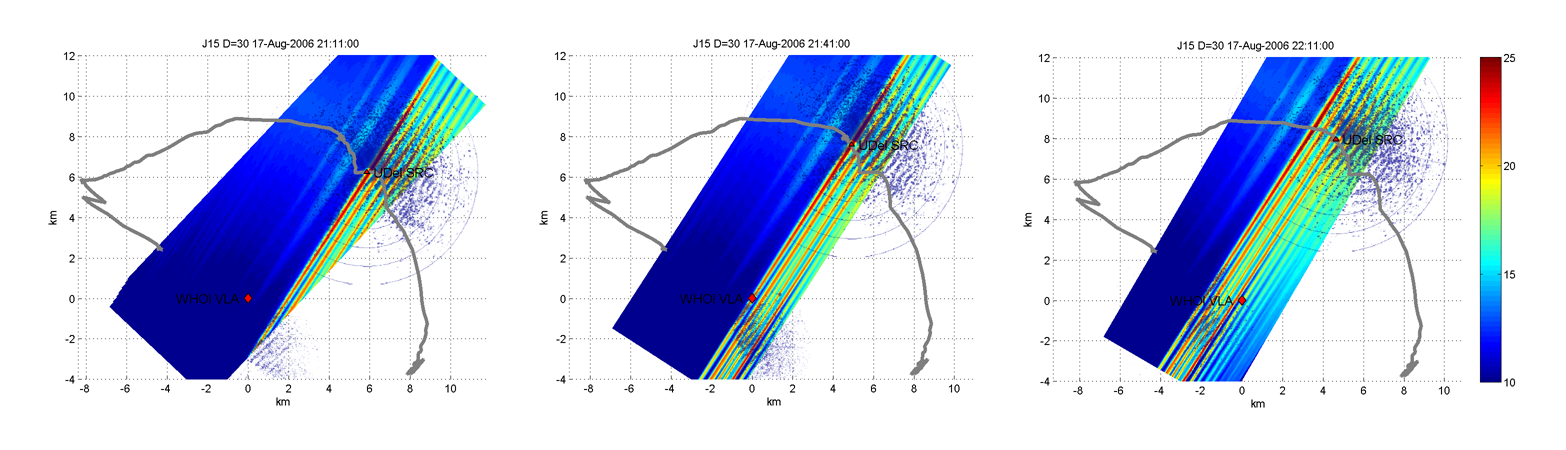
\includegraphics[width=\textwidth]{3D_interp_radar.png}\\
  %\caption{Reconstructed temperature field (depth = 30m) with radar image overlay at GMT21:11, 21:41 \& 22:11, Aug 17th.}
  %\label{fig: 3D_interp_radar}
%\end{figure}




\clearpage

\begin{figure}[H]
\centering
  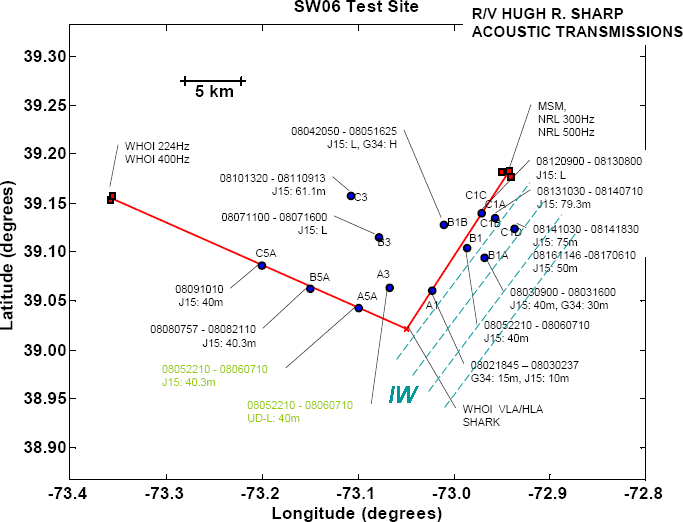
\includegraphics[width=\textwidth]{transmission1.png}
  \caption{Positions of the J15 acoustic source deployed from R/V Sharp during SW06 experiment. Some positions were chosen to vary the angle between the acoustic track and the IW propagation.}
  \label{fig:transmission}
\end{figure}


\begin{figure}[H]
  \centering
  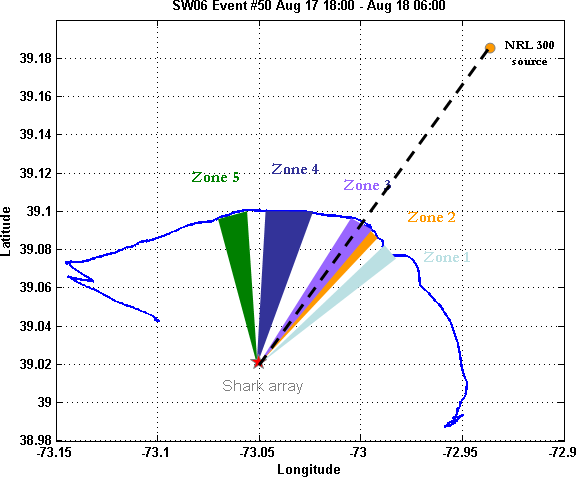
\includegraphics[width=\textwidth]{zones.png}
  \caption{Positions of the fixed and mobile acoustic sources.}\label{fig:zones}
\end{figure}


\begin{figure}[H]
\centering
  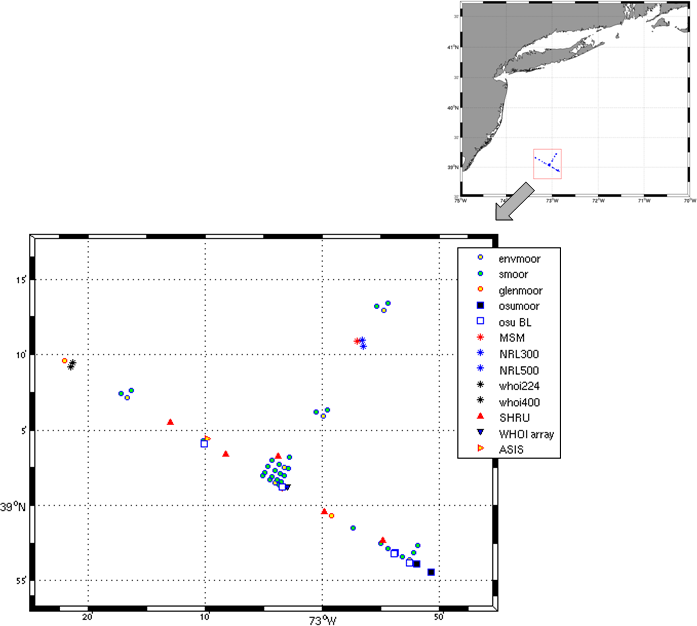
\includegraphics[width=\textwidth]{moorings_site.png}\\
  \caption{SW06 mooring locations}
  \label{fig:moorings}
\end{figure}



\begin{figure}[H]
\centering
  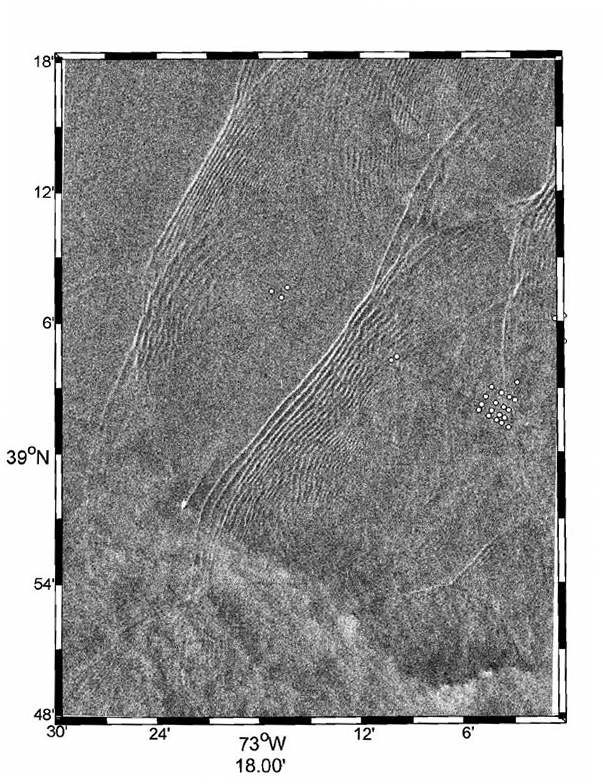
\includegraphics[width=\textwidth]{satellite.png}\\
  \caption{Radarsat observation from August 13, 2006. Some of the SW06
moorings are shown in the figure to provide scale.}
  \label{fig:satellite}
\end{figure}


\begin{figure}[H]
\centering
  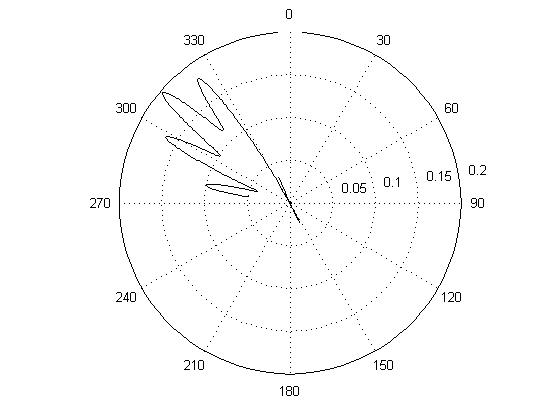
\includegraphics[width=\textwidth]{iw_direction.jpg}\\
  \caption{Calculated direction of dominant IW event observed based on 60 observed IW events}
  \label{fig:IW_dir}
\end{figure}

\begin{figure}
  \centering
  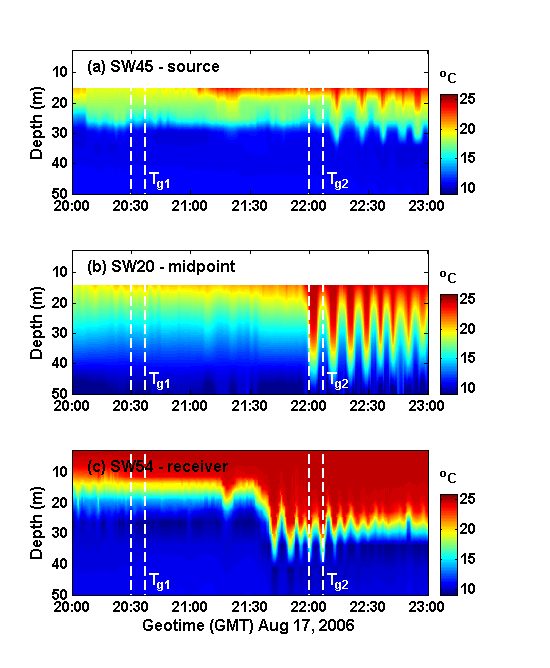
\includegraphics[width=\textwidth]{jasa2_temperature.png}
  \caption{Temperature profiles measured at (a) the acoustic source, (b) the midpoint between the source and receiver, and (c) at the Shark WVHLA during internal wave Event 50, August 17, 2006 from 20:00 to 23:00 GMT. $T_{g1}$ = 20:30 to 20:37 GMT and $T_{g2}$ = 22:00 to 22:07 GMT.}\label{fig:temp}
\end{figure}
